\chapter{Case Study}\label{cha:assembly}
In order to develop and test the model, we have chosen to focus on one representative case study. In this case study the robot is assembling an enclosed emergency stop button used in industrial environments, see Figure \ref{fig:button}. The assembly is presented in \cite{assembly} and has an associated video of the assembly\footnote{\url{http://www.youtube.com/watch?v=7JgdbFW5mEg}}. Please note that this is not the video used to extract the times for the tasks, so the times may differ from the ones used. Also, only the assembly of one stop button is performed in this thesis, not several as in this video.

This assembly is composed of 5 components; a top, a button, a nut, a switch and a bottom. A combination of components that is not the complete assembly we will call a sub-assembly. The button needs to be inserted in the top and then the nut needs to be screwed onto the underside of the button in order to secure it to the top. The switch needs to be mounted in the bottom and, lastly, the top part, with button and nut, needs to be mounted on the bottom with the switch. In Figure \ref{fig:assembly} we see the top-button-nut assembly to the right and the bottom-switch assembly to the left. Note that the screws in the figure are not part of the case study assembly.

\begin{figure}
\centering
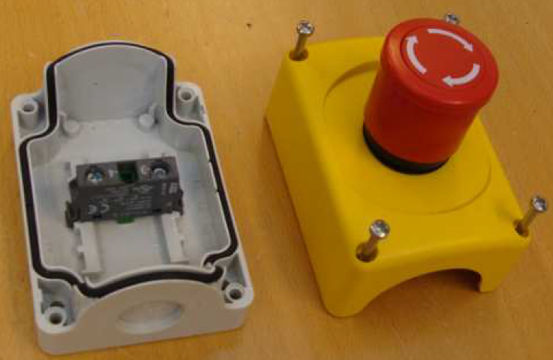
\includegraphics[width=\textwidth/3*2]{Figures/buttonbox.png}
\caption{Picture of the button used in the case study. The screws are not part of the case study assembly}
\label{fig:button}
\end{figure}

The assembly includes objects such as trays and fixtures. A tray is a holder where components reside until they are needed in the assembly. A fixture is a holder in which components can be put so that another components can be mounted on it.

21 steps have been identified as needed for the assembly and they are taken from a video of an existing assembly created by hand. For an illustration of the order of the assembly steps, see Figure \ref{fig:assembly} The steps are as follows:

\begin{description}
\item[Take top] Takes the top component from its tray

\item[Put top in fixture] Puts the taken top component in a fixture

\item[Take button] Takes the button component from its tray

\item[Mount button on top] Mounts the taken button component onto the top component in a fixture

\item[Angle top-button] Angles the sub-assembly that is the top and button component, from here on called top-button, so it can be supported by the other machine.

\item[Lift top-button, hold top button] Lifts the top-button by holding the button

\item[Lift top-button, support] Lifts the top-button by supporting the top from underneath

\item[Turn top-button] Turns the top-button by holding the button

\item[Take nut] Takes the nut from its tray

\item[Mount nut on top-button, hold] Mounts the nut on top-button while holding the button

\item[Mount nut on top-button, mount] Mounts the nut on the top-button holding and screwing the nut. The sub-assembly created by the top-button and the nut is here on after called top-button-nut

\item[Fixate top-button-nut] Fixates the top-button-nut using the side of a fixture in order to get it straight.

\item[Put top-button-nut in top tray] The top-button-nut is put in the top tray in order to put it away for a while to be picked up later.

\item[Take top-button-nut from top tray] Takes the top-button-nut from the top tray where it was previously put.

\item[Take bottom] Takes the bottom component from its tray.

\item[Put bottom in fixture] Puts the bottom component in a fixture.

\item[Take switch] Takes the switch component from its tray.

\item[Mount switch in bottom] Mounts the switch on the bottom in the fixture the bottom was put in. The sub-assembly created here will be called bottom-switch.

\item[Take bottom-switch] Takes the created bottom-switch from the fixture.

\item[Put bottom-switch on table] Puts the bottom-switch on the table.

\item[Mount top-button-nut on bottom-switch] Mounts the top-button-nut on the button-switch on the table.
\end{description}

\noindent Most of the steps are self explanatory, but there are a few steps which are quite special that might need some more explanation. In steps \textbf{Mount nut on top-button, hold} and \textbf{Mount nut on top-button, mount} the button component has been put in the hole of the top and needs to secured using the nut component. To do this something that is special for YuMi\textsuperscript\textregistered is utilized, both arms are used in order to mount the nut. This is done mid air with one arm holding the top-button by holding the button part, having it upside-down compared to how it was in the fixture, and with the other arm screwing the nut in place. The preparation for this starts at the end of step \textbf{Mount button on top}, where the sub-assembly top-button was just created, but the button is only loosely sitting in the hole of the top. The sub-assembly is angled in task \textbf{Angle top-button} about 45$^\circ$ in order to create a gap under the sub-assembly so the other arm can reach under the sub-assembly and help lift it from the fixture in tasks \textbf{Lift top-button, support} and \textbf{Lift top-button, hold top button}. Finally the top-button is rotated by only holding it with one arm in the button part of the sub-assembly and are now ready for the nut to be mounted.
It should be noted that since the operations of lifting the top-button and mounting the nut takes two arms and we have here split the operations into two tasks each, one for each arm, the tasks \textbf{Mount nut on top-button, hold} and \textbf{Mount nut on top-button, mount} needs to be performed at the same time. The same goes for  \textbf{Lift top-button, support} and \textbf{Lift top-button, hold top button}.

As mentioned before, the steps listed are taken from a video of an assembly. This makes the times used in the case study approximated. First the times where approximated using seconds as the unit of time. But it showed to be hard to approximate some of the tasks as they sometimes where under 1 second in time. Because of this and to get better print outs of the assembly using \texttt{SchedPrinter} (see appendix \ref{app:tool_manuals}) we multiplied the times we could estimate well from the video by 5 and approximated the other tasks as well as we could. This means that the real times for the tasks in the case study, and in the files mentioned in appendix \ref{app:tool_manuals}, are $1/5$ of the time presented. Because of this, comparing the time from the solvers with the time of the manual assembly is harder. We had to approximate the time of the manual assembly using the times we have approximated. By analysing the video and using the approximated times we got a time of 516 time units for the manual assembly.

\begin{landscape}
\begin{figure}
\documentclass{standalone}
\usepackage{standalone}
\begin{document}
\tikzstyle{task} = [rectangle, minimum width=3cm, minimum height=1cm, text centered, draw=black]
\tikzstyle{arrow} = [thick,->,>=stealth]
\begin{tikzpicture}[node distance=2cm]
\node (1) [task] {Take top};
\node (2) [task, right of=1, xshift=2.5cm] {Put top in fixture};

\node (3) [task, below of=1] {Take button};
\node (4) [task, below of=2] {Mount button on top};

\node (5) [task, xshift=2.5cm, right of=4] {Angle top-button};

\node (6) [task, right of=5, xshift=3cm, yshift=1cm] {Lift top-button, hold};
\node (7) [task, below of=6] {Lift top-button, support};

\node (8) [task, right of=7, xshift=3.5cm, yshift=1cm] {Turn top-button};

\node (10) [task, below of=8] {Mount ring, hold};
\node (11) [task, below of=10] {Mount ring, mount};

\node (9) [task, below of=11] {Take ring};

\node (12) [task, left of=11, xshift=-4cm, yshift=1cm] {Fixate top-button-ring};

\node (13) [task, left of=12, xshift=-9.5cm] {Put top-button-ring in top tray};
\node (14) [task, below of=13] {Take top-button-ring from top tray};

\node (15) [task, below of=9, yshift=-1.5cm] {Take switch};
\node (16) [task, left of=15, xshift=-3cm] {Mount switch};

\node (17) [task, below of=15] {Take bottom};
\node (18) [task, below of=16] {Put button in fixture};

\node (19) [task, left of=16, xshift=-3.5cm] {Take button-switch};

\node (20) [task, left of=19, xshift=-5cm] {Put bottom-switch on table};

\node (21) [task, above of=20] {Mount top-button-ring on bottom-switch};

\draw [arrow] (1) -- (2);
\draw [arrow] (3) -- (4);
\draw [arrow] (2) -- (4);
\draw [arrow] (4) -- (5);
\draw [arrow] (5) -- (6);
\draw [arrow] (5) -- (7);
\draw [arrow] (7) -- (8);
\draw [arrow] (6) -- (8);
\draw [arrow] (8) -- (10);
\draw [arrow] (10) -- (12);
\draw [arrow] (9) -- (11);
\draw [arrow] (11) -- (12);
\draw [arrow] (12) -- (13);
\draw [arrow] (13) -- (14);
\draw [arrow] (15) -- (16);
\draw [arrow] (17) -- (18);
\draw [arrow] (18) -- (16);
\draw [arrow] (16) -- (19);
\draw [arrow] (19) -- (20);
\draw [arrow] (20) -- (21);
\draw [arrow] (14) -- (21);

\end{tikzpicture}
\end{document}
\caption{The case study assembly}
\label{fig:assembly}
\end{figure}
\end{landscape}

%\documentclass{standalone}
\begin{document}
\begin{table}
\centering
\begin{tabular}{c|l|p{6cm}}
Step & Name                                  & Comment\\
\hline
1   & Take top                               & Takes the top component from its tray\\
2   & Put top in fixture                     & Puts the taken top component and puts it in a fixture\\
3   & Take button                            & Takes the button component from its tray\\
4   & Mount button on top                    & Mounts the taken button component onto the top component in a fixture\\
5   & Angle top-button                       & Angles the assembly that is the top and button component, from here on called top-button\\
6   & Lift top-button, hold top button       & Lifts the top-button by holding the button\\
7   & Lift top-button, support               & Lifts the top-button by supporting the top from underneath\\
8   & Turn top-button                        & Turns the top-button by holding the button\\
9   & Take ring                              & Takes the ring from its tray\\
10  & Mount ring on top-button, hold         & Mounts the ring on top-button by holding the button\\
11  & Mount ring on top-button, mount        & Mounts the ring on the top-button holding and screwing the ring. The assembly created by thetop-button and the ring is here on after called top-button-ring\\
12  & Fixate top-button-ring                 & Fixates the \\
13  & Put top-button-ring in top tray        &\\
14  & Take top-button-ring from top tray     &\\
15  & Take bottom                            &\\
16  & Put bottom in fixture                  &\\
17  & Take switch                            &\\
18  & Mount switch in bottom                 &\\
19  & Take bottom-switch                     &\\
20  & Put bottom-switch on table             &\\
21  & Mount top-button-ring on bottom-switch &\\
\end{tabular}
\caption{Steps in case study}\label{tab:assembly_steps}
\end{table}
\end{document}